% Drawing 154/02-8 -- folder 154, batch 02, archive page 30 (PDF page 31).
% Transcription: figure, en haut à droite : une carte à faces quadrangulaires tracée en vert foncé, son dual en vert clair, les faces hachurées au crayon ; un sommet $s$ marqué d'un point, une arête fléchée $\vec{a}$ de $s$ vers $t$, et les orientations $\omega_s$, $\omega_t$ figurées par de petites flèches courbes ; un cercle brun entoure un sommet de la carte
% Kind: quadrangulated map with its dual. Method 2 (schematic redraw from the facsimile). Status: partial.
% Notes: Top right: a map with quadrangular faces in dark green, its dual in light green (yellow-green on the facsimile), the faces hatched in pencil; a vertex s marked with a point, an arrowed edge a from s to t, the orientations omega_s, omega_t as small curved arrows (drawn as labels), and a brown circle round a vertex of the map. The edges are drawn as on the page, but the outer edges run off unevenly and the faces are not all closed on the sheet, so the map is not encoded; the pencil hatching and the dashed pencil edges are left out.
% Coordinates: 1 unit = 1 mm = 1/100 of the crop width (bbox in page fractions: [0.551, 0.085, 0.814, 0.316]).
% Redrawn by Claude (claude-opus-5-5), issue #73, 2026-11-07; not checked by a human; not compiled (no TeX in the session).
% Rights: reproduces part of the work -- behind RENDER_TRANSCRIPTS, never published by itself.
\documentclass[tikz,border=3pt]{standalone}
\usepackage{amsmath,amssymb}
\usetikzlibrary{patterns,arrows.meta}
\tikzset{Or/.style={orange!90!black}, Ye/.style={yellow!80!orange}, Lg/.style={green!60!black!70}, Dg/.style={green!45!black}, Br/.style={brown!80!black}, Rd/.style={red!85!black}, Bl/.style={blue!70!black}, Gy/.style={black!40}, pencil/.style={black!45}, struck/.style={black!35}, mark/.style={circle,draw,inner sep=1.3pt}, pt/.style={circle,fill,inner sep=0.9pt}, opt/.style={circle,draw,fill=white,inner sep=1.1pt}}
\begin{document}
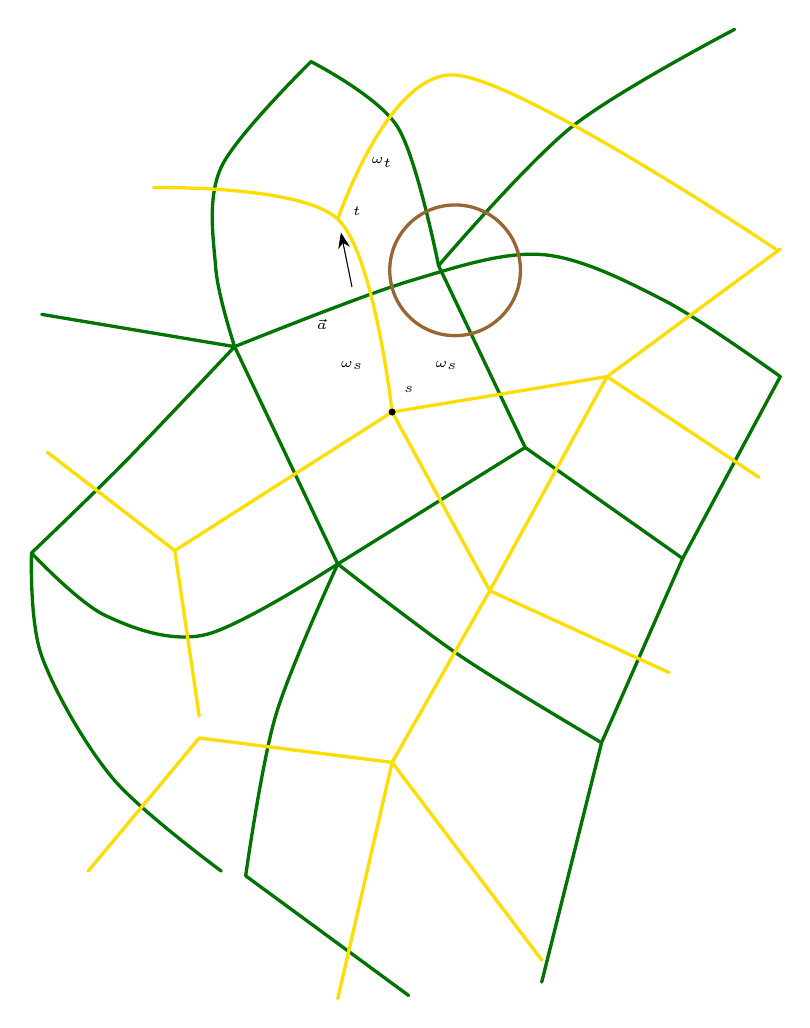
\begin{tikzpicture}[x=1mm,y=1mm,line cap=round,line join=round,font=\scriptsize]
\draw[Dg,very thick] (3.4,-35.9) -- (27.9,-40);
\draw[Dg,very thick] plot[smooth, tension=0.55] coordinates {(37.6,-3.8) (26.2,-17.2) (25.5,-30) (27.9,-40)};
\draw[Dg,very thick] plot[smooth, tension=0.55] coordinates {(37.6,-3.8) (48.6,-12.1) (53.8,-29.7)};
\draw[Dg,very thick] plot[smooth, tension=0.55] coordinates {(27.9,-40) (50,-31.7) (66.9,-28.3) (82.4,-34.1) (97.2,-43.8)};
\draw[Dg,very thick] (53.8,-29.7) -- (64.8,-52.8);
\draw[Dg,very thick] plot[smooth, tension=0.55] coordinates {(53.8,-29.7) (70.7,-12.1) (91.4,0.3)};
\draw[Dg,very thick] (97.2,-43.8) -- (84.8,-66.9);
\draw[Dg,very thick] (84.8,-66.9) -- (64.8,-52.8);
\draw[Dg,very thick] (84.8,-66.9) -- (74.5,-90.3);
\draw[Dg,very thick] (74.5,-90.3) -- (66.9,-120.7);
\draw[Dg,very thick] (64.8,-52.8) -- (41,-67.6);
\draw[Dg,very thick] (41,-67.6) -- (27.9,-40);
\draw[Dg,very thick] plot[smooth, tension=0.55] coordinates {(2.1,-66.2) (13.8,-54.8) (27.9,-40)};
\draw[Dg,very thick] plot[smooth, tension=0.55] coordinates {(2.1,-66.2) (11.4,-74.1) (24.1,-76.6) (41,-67.6)};
\draw[Dg,very thick] plot[smooth, tension=0.55] coordinates {(41,-67.6) (33.1,-86.9) (29.3,-107.2)};
\draw[Dg,very thick] plot[smooth, tension=0.55] coordinates {(41,-67.6) (56.6,-79.3) (74.5,-90.3)};
\draw[Dg,very thick] plot[smooth, tension=0.55] coordinates {(2.1,-66.2) (3.4,-79.3) (12.4,-94.8) (26.2,-106.6)};
\draw[Dg,very thick] (29.3,-107.2) -- (50,-122.4);
\draw[Ye,very thick] (47.9,-48.3) -- (20.3,-65.9);
\draw[Ye,very thick] (47.9,-48.3) -- (75.2,-43.8);
\draw[Ye,very thick] plot[smooth, tension=0.55] coordinates {(47.9,-48.3) (41,-23.8) (17.6,-19.8)};
\draw[Ye,very thick] plot[smooth, tension=0.55] coordinates {(41,-23.8) (55.9,-5.5) (96.6,-27.6)};
\draw[Ye,very thick] (47.9,-48.3) -- (60.3,-71);
\draw[Ye,very thick] (60.3,-71) -- (75.2,-43.8);
\draw[Ye,very thick] (60.3,-71) -- (47.9,-92.8);
\draw[Ye,very thick] (60.3,-71) -- (83.1,-81.4);
\draw[Ye,very thick] (75.2,-43.8) -- (94.5,-56.6);
\draw[Ye,very thick] (75.2,-43.8) -- (97.2,-27.6);
\draw[Ye,very thick] (20.3,-65.9) -- (4.1,-53.4);
\draw[Ye,very thick] (20.3,-65.9) -- (23.4,-86.9);
\draw[Ye,very thick] (47.9,-92.8) -- (23.4,-89.7);
\draw[Ye,very thick] (23.4,-89.7) -- (9.3,-106.6);
\draw[Ye,very thick] (47.9,-92.8) -- (41,-122.8);
\draw[Ye,very thick] (47.9,-92.8) -- (66.9,-117.9);
\node[pt] at (47.9,-48.3) {};
\node[inner sep=1pt] at (50,-45.5) {\tiny $s$};
\node[inner sep=1pt] at (43.4,-22.8) {\tiny $t$};
\draw[-{Stealth[length=2mm]}] (42.8,-32.4) -- (41.4,-25.5);
\node[inner sep=1pt] at (39,-37.2) {\tiny $\vec a$};
\node[inner sep=1pt] at (42.8,-42.4) {\tiny $\omega_s$};
\node[inner sep=1pt] at (54.8,-42.4) {\tiny $\omega_s$};
\node[inner sep=1pt] at (46.6,-16.6) {\tiny $\omega_t$};
\draw[Br,very thick] (55.9,-30.3) circle[radius=8.3];
\end{tikzpicture}
\end{document}
